\section{Aggregated subsector dependency network}
\label{sec:subsector_network}

Asset-level networks can be difficult to interpret when many share classes and sectors are present. The aggregated subsector dependency network converts ticker-level dependencies into a mesoscopic map. Nodes represent subsectors and edges summarize average retained dependency strength between subsectors. This is analogous to sector or country aggregation maps used in the financial dependency literature, but adapted to the Brazilian equity universe \cite{raddant_dimatteo_2023}.

Figure~\ref{fig:subsector_network} presents the resulting network. The network contains 22 subsectors and 66 edges, with density 0.2857. The mean edge dependency is 0.0566 and the median edge dependency is 0.0561. These values are lower than typical raw asset-level correlations, which is expected because the network summarizes filtered and aggregated dependencies rather than direct pairwise asset correlations.

The top-degree subsector is Retail, indicating broad direct connectivity in the aggregated dependency map. Electric Utility has the highest betweenness, suggesting that it occupies a bridge-like position in the mesoscopic topology. Apparel and Footwear has the highest weighted degree, reflecting stronger dependency intensity across its retained connections. These summaries help translate the ticker-level PMFG topology into economic language.

The subsector network also provides a bridge to forecasting. If network topology contains information beyond univariate volatility persistence, then node-level or group-level centrality measures may help explain future volatility regimes. The forecasting section tests this idea in a conservative first experiment.


\begin{center}
\captionof{table}{Aggregated subsector network summary.}
\label{tab:subsector_summary}
\resizebox{\linewidth}{!}{%
\begin{tabular}{rrrrrlll}
\toprule
Subsectors & Edges & Density & Mean edge dep. & Median edge dep. & Top degree & Top betweenness & Top weighted degree \\
\midrule
22 & 66 & 0.2857 & 0.0566 & 0.0561 & Retail & Electric Utility & Apparel and Footwear \\
\bottomrule
\end{tabular}}
\end{center}

\begin{center}
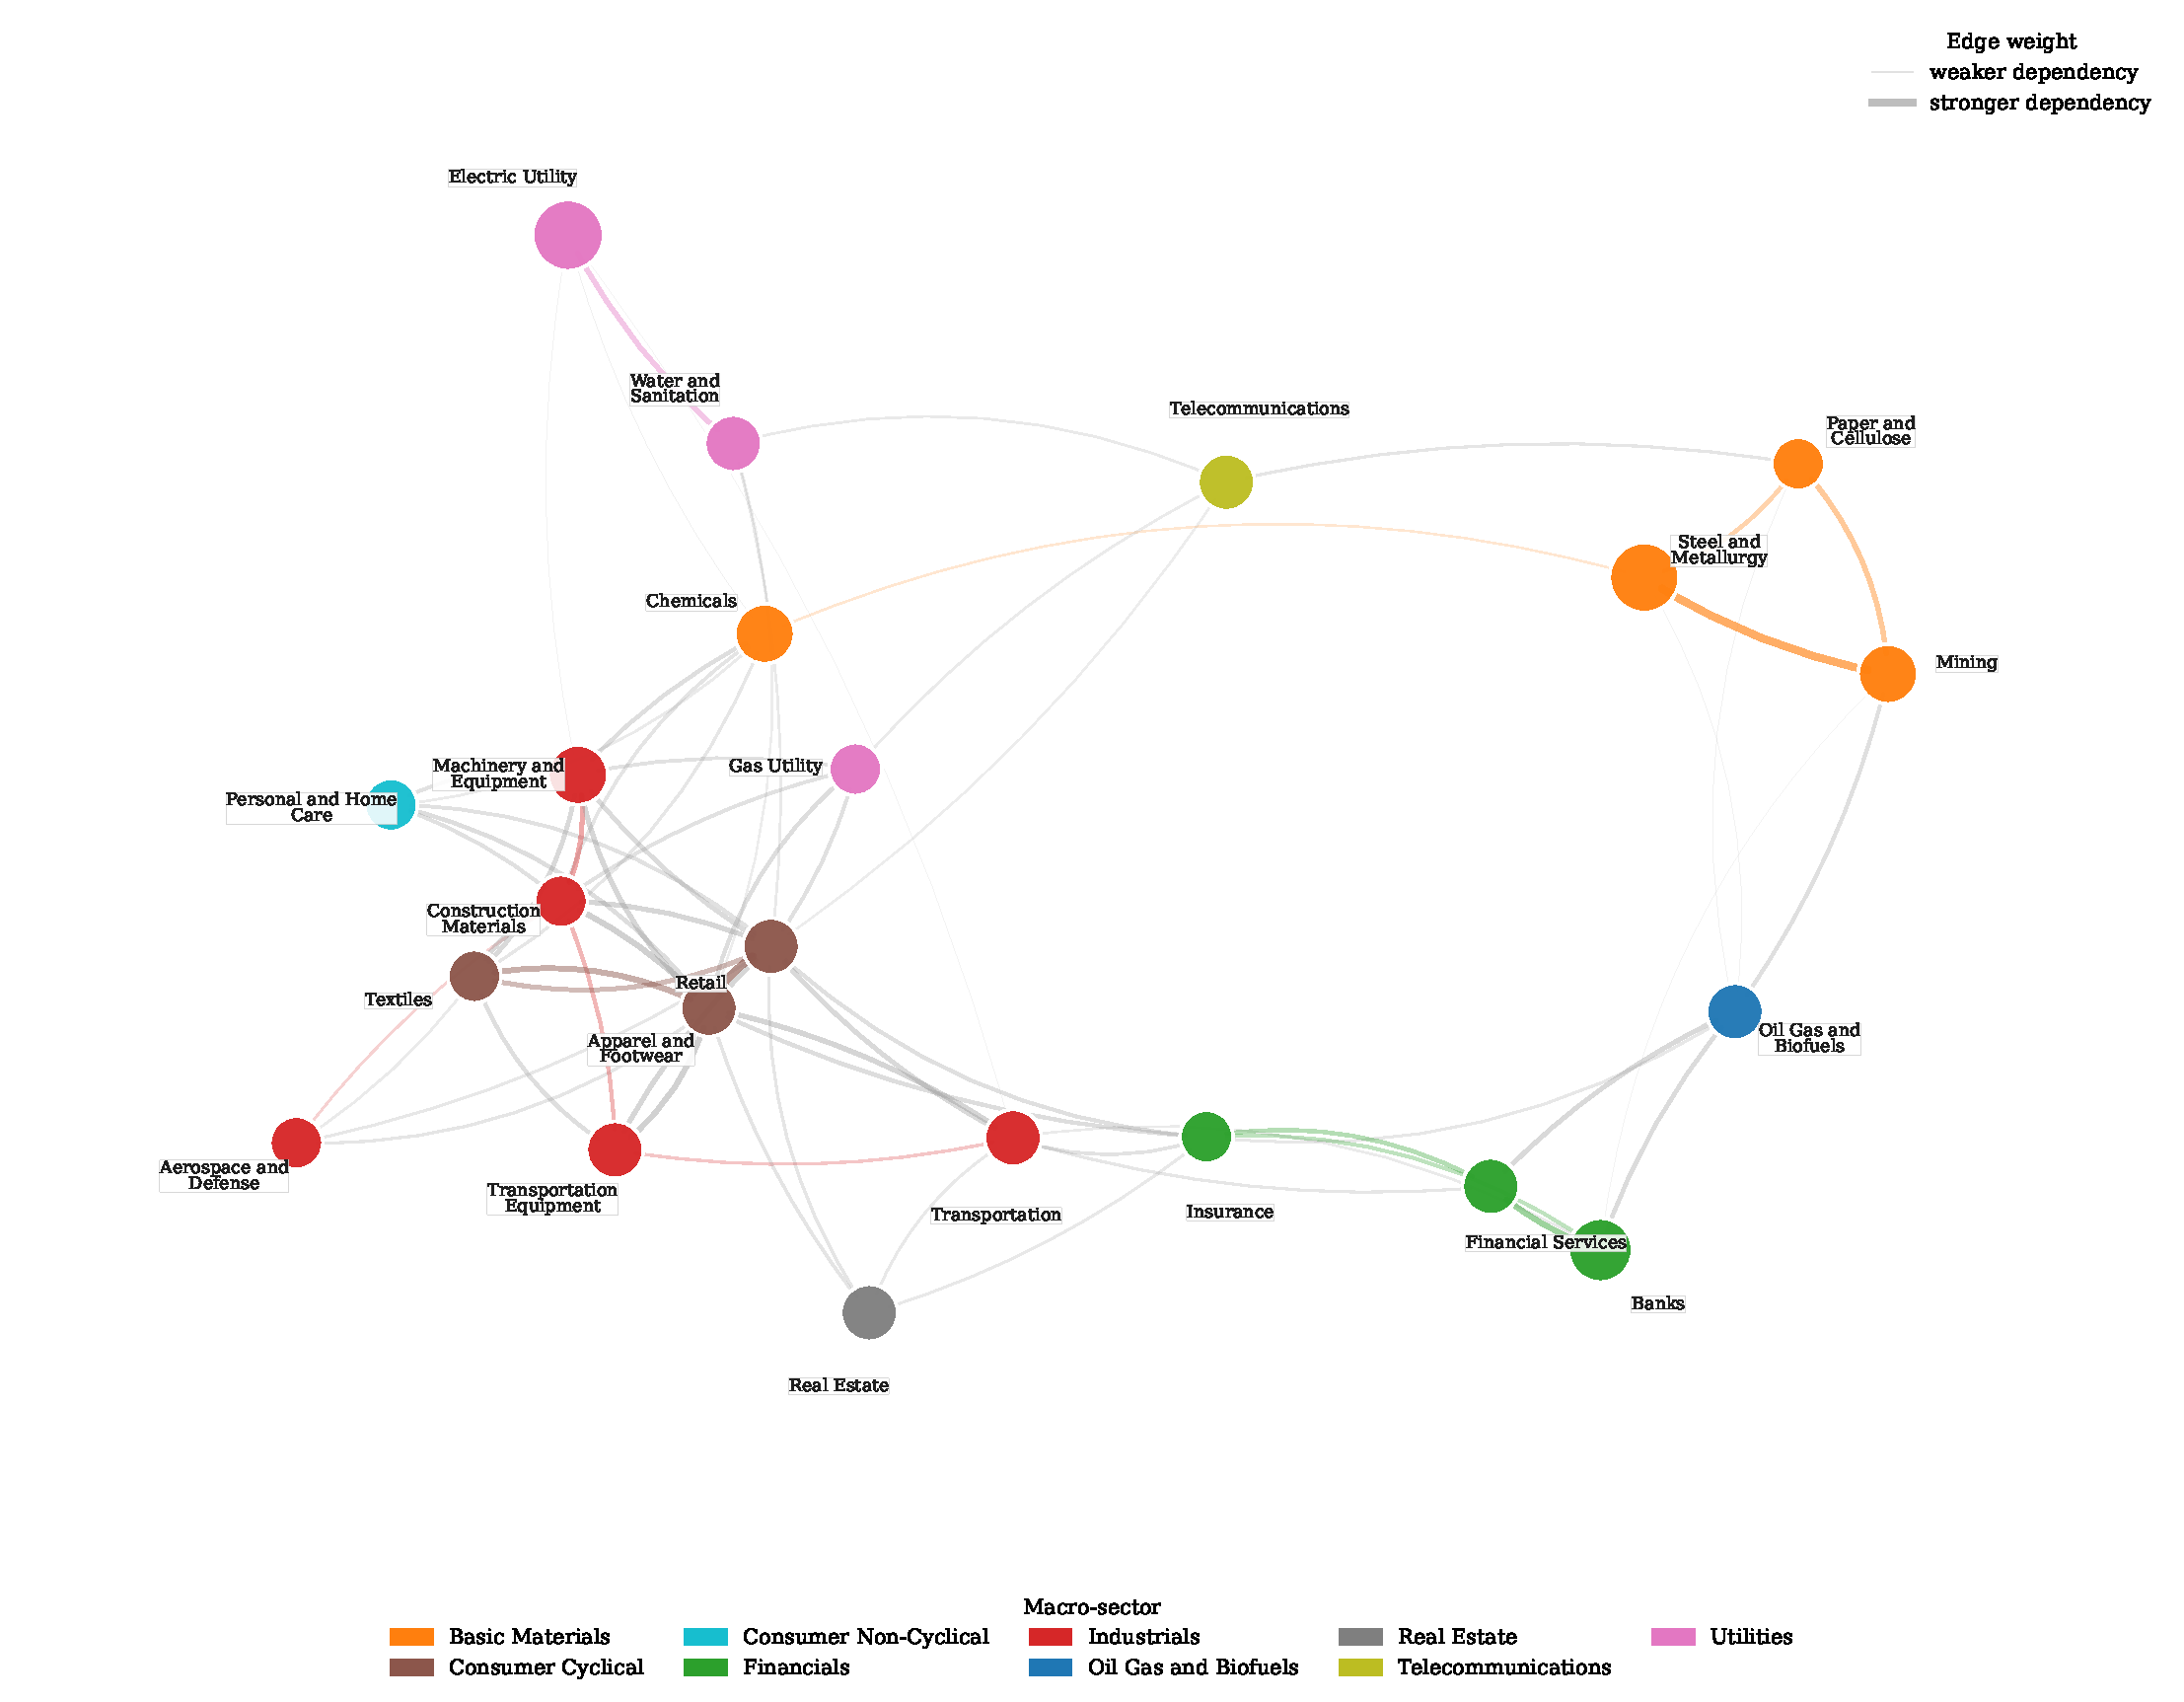
\includegraphics[
  width=0.92\linewidth,
  height=0.58\textheight,
  keepaspectratio
]{images/figure_15_subsector_dependency_network.pdf}
\captionof{figure}{Aggregated subsector dependency network. Asset-level dependencies are summarized into subsector-level connections, providing a mesoscopic view of the Brazilian equity market.}
\label{fig:subsector_network}
\end{center}

